% simple.tex -- Yaser Alkayale Thesis Taken From Vlado Keslj

\documentclass[12pt]{dalthesis}

\usepackage[algochapter,ruled,vlined,longend,linesnumbered,resetcount]{algorithm2e}
\usepackage{mathtools}
\usepackage[T1]{fontenc}
\usepackage{siunitx}
\usepackage{tikz} % To generate the plot from csv
\usepackage{pgfplots}
\usepackage{filecontents}
\usepackage{graphicx}
\usepackage{amsmath}
\usepackage{subcaption}
\usepackage{siunitx}
\usepackage{natbib}
\usepackage{amssymb}

\captionsetup{compatibility=false}

\newcommand*{\Value}{\frac{1}{2}x^2}
\newcommand*{\kmeans}{\textsc{K-Means} } %kmeans with space
\newcommand*{\kmeansn}{\textsc{K-Means}} %kmeans with no space

\usepgfplotslibrary{external}
\tikzexternalize{yaser_thesis}
\pgfplotsset{compat=newest} % Allows to place the legend below plot
% \usepgfplotslibrary{units} % Allows to enter the units nicely

\sisetup{
  round-mode          = places,
  round-precision     = 2,
}

% These will help for absolute value math operators
\DeclarePairedDelimiter\abs{\lvert}{\rvert}
\DeclarePairedDelimiter\norm{\lVert}{\rVert}
\DeclareMathOperator*{\argmin}{argmin}

% This is where all the images are used.
\graphicspath{ {images/} }

\begin{document}

% Swap the definition of \abs* and \norm*, so that \abs
% and \norm resizes the size of the brackets, and the 
% starred version does not.
\makeatletter
\let\oldabs\abs
\def\abs{\@ifstar{\oldabs}{\oldabs*}}
\let\oldnorm\norm
\def\norm{\@ifstar{\oldnorm}{\oldnorm*}}
\def\BState{\State\hskip-\ALG@thistlm}
\makeatother

\title{\kmeans Clustering, An Attempt At An Improved Seeding Process} %TODO: Change the title.
\author{Yaser Alkayale}
\bcshon  %Sets it to honours variant
\degree{Bachelor's of Computer Science, Honours}
\degreeinitial{B.C.Sc.}
\faculty{Computer Science}
\dept{Faculty of Computer Science}
\defencemonth{April}\defenceyear{2018}
\dedicate{This thesis is in dedication to my grandfather whom I was named after.}

\nolistoftables
\nolistoffigures

\frontmatter

\begin{abstract}
  Clustering is a well-known task that has been studied and used for decades. The idea is to take a set of items and group them into a number of clusters based on a similarity measure. \kmeans, although named differently back then, was proposed in 1957 by Stuart Lloyd and is one of the most widely used clustering algorithms and is still used today for its reasonably fast heuristic to find the clusters based on the Lloyd algorithm and more recent developments in that area. \kmeans has two main parts to clustering, the initial seeding process and the iteration process. The seeding process picks $k$ initial seeds as cluster centres, and highly affects the accuracy of the final result in the algorithm. The iteration process dominates running time to move the centres around until it converges to an optimum. In this paper, we discuss a new method of the seeding process that gives us more accurate seeds to start the algorithm. 
  %TODO: Add this later. We also discuss a novel approach to find an approximation of the correct number of clusters for a given dataset.

\end{abstract}



\begin{acknowledgements} 
  A sincere thank you to my supervisor Dr. Norbert Zeh. Without his assistance, this project would not have seen the day of light. Thank you to Dr. Vlado Keselj who made himself available when we needed to consult with him. Also big thank you to Arazoo who was with me from the beginning, and went through my ideas with me.
\end{acknowledgements}

\mainmatter

\chapter{Introduction \& Background}
Clustering is the task of grouping certain things into separate or overlapping groups based on a similarity criteria. Clustering problems arise in many domains like
natural language processing \citep{ravichandran2005randomized},
bioinformatics \citep{edgar2010search}
crash report analysis \citep{soto2016machine}, 
and vehicle navigation \citep{maio1996dynamic}.
The notion of what is a good cluster highly depends on the domain and application at hand. Many clustering techniques like hierarchical clustering \citep{corpet1988multiple}
and graph-based ones \citep{schaeffer2007graph}
exist, each serving a different purpose and are practical for different clustering tasks. \kmeans clustering continues to be one of the most popular clustering algorithms for it's simplicity of implementation and relative efficiency \citep{jain2010data}.

Different clustering algorithms are suited for different tasks. Some of them, like \kmeans, fit a given dataset into a given number of disjoint sets. Other algorithms allow points to belong to multiple clusters and are useful in applications like community clustering on social media graphs \citep{epasto2017ego}. In other instances, clustering is used on datasets where the number of clusters is unknown; for example, clustering images of people using facial recognition \citep{schroff2015facenet}. The effectiveness of a given algorithm is determined by domain it is being used in and the problem at hand.

Formally, \kmeans is the problem where one is given a set of $n$ points in $d$-dimensional space, $\mathbb{R}^d$, and a number $k$. The goal is to split the $n$ points into $k$ disjoint clusters, minimizing the cost function $\phi$, the sum of distances of each point to its cluster centre. \kmeans does especially well, in terms of speed and accuracy, on convex shaped clusters as it minimizes the sum of distances of all points to their belonging cluster centres. However, it struggles to perform well in terms of accuracy and running time when clusters are not convex shaped or $k$ is not the right number of actual clusters in the dataset.

Solving \kmeans exactly is known to be NP-hard, and that is why heuristics like Lloyd's \citep{1056489} iterations were introduced to give us an approximation of the solution by using local search. Lloyd is still the most widely used iterations process for its simplicity of implementation. It has been stated that \kmeans ``is by far the most popular clustering algorithm used in scientific and industrial applications'' \citep{clusteringservey}. A locally optimal solution is good enough in most cases, allowing us to have meaningful clusters in a reasonable amount of time. That, in addition to simplicity of implementation, makes \kmeans a good option in a lot of cases, hence the popularity.

While \kmeans is widely used for its proven practical performance, it is not perfect for many use cases. The algorithm can give highly inaccurate clusters if the incorrect number $k$ is given to the algorithm. This is due to the nature of the algorithm forcing all the points into $k$ clusters. Another problem with the algorithm is that it produces convex shaped clusters, which inherently produces highly inaccurate clusters if the correct clusters are not convex shaped. The algorithm also struggles when there is a lot of noise\footnote{Note: Noise in this context is referring to the overlap of multiple clusters, where it becomes difficult to separate points if they are at the edges of two or more clusters.} in the data because having points between two clusters makes it difficult to force them into only one as membership becomes unclear. Inputting the incorrect number $k$ to the algorithm and/or having incorrect data leads to the algorithm struggling with running time and accuracy.

In this paper, we introduce a new way to seed the \kmeans algorithm which turned out to be no better than randomly seeding \kmeans. The ideas of the algorithm and its pseudocode are outlines below along with results. We also explain the C++ implementation of the algorithm and ways it can be used for further development and research.


\section{The \kmeans algorithm.}
The \kmeans algorithm is simple and relatively efficient as it minimizes the objective function locally depending on its seeds.
Here are the steps of the algorithm \cite{arthur2007k}. Input is assumed to be the dataset $X$ and the number of clusters required $k$:

\begin{enumerate}
  \item Pick $k$ points arbitrarily at random from $X$.
  \item Point $p$ in $X$ belongs to cluster $C_i$ if $p$ is closer to $c_i$ than it is to $c_j$ for all $j \neq i$, $1 \leq i,j \leq k$
  \item For $i$ in \{1...k\} compute new centre $c_i = \frac{1}{\abs{C_i}}\sum_{x \in C_i}x$
  \item Repeats steps 3 and 4 until centres do not change\footnote{In reality, the centres rarely ever stop changing, so heuristics need to be used to stop the algorithm in reasonable time.}.
\end{enumerate}

Of course, the algorithm may not always converge in a reasonable amount of time, so a stop condition is used when the centres do not change beyond a threshold at a certain point. Another heuristic that is used is to set a maximum number of iterations to run.

\section{Seeding Process}

The seeding process of the \kmeans algorithm is crucial to the accuracy of the output because while the iterations converge the centres to an optimum, it is localized to the regions constrained by the initial seeds \citep{arthur2007k}.
Many new approaches to pick initial seeds like \kmeansn++ \citep{arthur2007k}, and \kmeansn|| \citep{bahmani2012scalable} have been introduced which help pick seeds that converge faster. It has been experimentally proven that having a better seeding process improves the algorithm by both lowering the objective function of the algorithm, and allowing it to converge faster with less iterations and running time \citep{arthur2007k}.

Given the dataset $X$ and the number $k\leq \abs{X}$ to cluster, \kmeans picks $k$ points from the dataset uniformly at random. The Lloyd method does not specify any way of picking the initial seeds. It only required $k$ seeds to run and converge an a local optimum. The widely used method of seeding \kmeans  is to do it uniformly at random. Picking the seeds uniformly at random helps works because allows the iterations to start at some points, but doesn't help in minimizing the objective function in any meaningful way. Newer ways have been introduced that substantially improve both running time and accuracy of the algorithm.

It it important to note here that we are only able to compute an optimum, not the optimal solution because the problem is NP-hard\cite{mahajan2009planar}. This means that we are unable to compute the optimal solution of any large enough instances in reasonable time. For that, a heuristic, i.e. Lloyd's iterations, are used to compute reasonably accurate centres in time.

\subsection{\kmeansn++: A Better Seeding Process}
\kmeansn++ uses an intuitive way to seed the initial clusters of the algorithm by trying to pick seeds that are as far apart as possible. This is done by giving a higher probability for points that are further away from the ones already picked. The way it works is that we pick a random initial point, and then given a higher probability of picking a point disproportional to its distance the seeds already picked, until k seeds are picked\cite{arthur2007k}.

\kmeansn++ works well because by skewing the probabilities of picking seeds towards ones that are farther from the already picked ones, we are helping pick seeds in different clusters in the dataset. It works especially well because a concentration of points already has a high probability of picking at least one of them picked, and lowering the probabilities for points that are close to ones that have already been chosen allows us to probabilistically almost ensures having a point from each cluster.

\kmeansn++ works very well because it about evenly distributes the initial seeds in the dataset. It is important to note that the probabilistic model still gives a chance for any of the points to be chosen, just some higher than others. This is crucial as we are merely making ``good guesses'' as to what the initial seeds should be, but are in no way trying to compute the ``perfect seeds'' because that would be solving the \kmeans problem, and as discussed earlier, that is NP-hard.

From my research, \kmeansn++ seams to be the best scientifically proven way to seed the \kmeans algorithm. There, however, have been improvements on the \kmeansn++ seeding algorithm like \kmeansn|| which improves the algorithm by making it parallelizable for very large datasets. 


\section{Iterations}

The iteration process of the \kmeans clustering algorithm dominates the running time of the algorithm. Running time for random seeding is $O(k)$, while the iterations run in $cO(nkd)$. Depending on how quickly the iterations converge, the $c$ constant may be very large. Even with \kmeansn++, running time for seeding is $cO(nkd)$ but $c=O(k)$, and in practice is still dominated by the iterations running time. 
Different approaches have been used to run the iterations and converge the centres. These approaches have had high success in reducing the running time of the algorithm \cite{alsabti1997efficient}. However, the implementation of these methods are not as simple as Lloyd's iterations, making them not as widely used.  

\section{Objective Function}
The objective function, $\phi$, of the clustering task determines based on what the points are being grouped. In most tasks, including in everything discussed in this paper, the objective function is the sum of squared euclidean distances\footnote{Note: Here squared distance is used because comparing distances and the square maintains the ordering of the points and saves a large amount of computational time as square rooting numbers is computationally costly.}
of all the points to their cluster centres. More formally expressed as:
$$\phi = \sum_{x\in X} \min_{c\in C}\abs{ x-c}^2$$

This objective function is the reason why \kmeans inherently produces convex shaped clusters as it tries to minimize the distance of each point to its cluster centre. If a point is marginally closer to a centre than another, it is grouped with the closer one. Geometrically this disallows concave shapes of any cluster. This is good for datasets where clusters are geometrically convex or close to it, but poses problems where the underlying data is not convex or is not clearly separable.

\section{Difficulties}

\kmeans clustering is very good at clustering well-separated convex clustered where k the number of clusters in known or accurately measured in advance. However, this is very rarely the case. Another issue with \kmeans is that it fits every point into a single cluster. This means that a point has no way of belonging to different clusters at the same time. 


\chapter{Improved Seeding Process?}

Here we introduce the new seeding process for \kmeans. The basic idea is to run the randomized seeding process $T$ times, each time running a small, $S$, number of iterations which produce a set of $k$ centres that have not converged. We then take the ($T*K$) centres, and cluster those into $k$ clusters.


\section{The Algorithm Pseudocode}

\begin{algorithm}[H]
  \caption{Consensus Seeding. Note: kmeans.cluster is a function that takes three values, the dataset, the number $k$ of clusters and an optional value, the maximum  number of iterations for the algorithm. The maximum number of iterations is set to infinity by default.}
  \SetAlgoLined
  \BlankLine
  \SetKwInOut{Input}{Input}
  \SetKwInOut{Output}{Output}
  \BlankLine
  \Input{$k$: the number of clusters\\ 
        dataset: the $d$ dimentional dataset to be clustered\\
        $r$: the number of rounds to run for the consensus\\
        $m$: the maximum number of iterations to use for each round}
  \Output{List of $k$ cluster centre seeds}
  runCentres $\leftarrow$ \{\}\;
  \For{$i=0...r$}{
    $runCentres \leftarrow runCentres \cup kmeans.cluster(dataset, k, m)$\;
  }
  \Return kmeans.cluster(runCentres,k)
\end{algorithm}

\section{Analysis \& Datasets}


To analyze the performance of the algorithm we ran it on 3 different datasets. The Cloud Data Set has $1025$ values in $10$ dimensions, and they represent the values for cloud cover \citep{cloud}. The Spambase Dataset consists of $4601$ values in $58$ dimensions, and it represents numerical representations for spam emails \citep{spam}. The Dimred dataset comes from a dimensionality reduced textual corpora of crash reports, it has $108,669$ values in $2$ dimensions.

Tables \ref{table:cloud}, \ref{table:spam}, and \ref{table:dimred} show experimental results for the accuracy and running time of the algorithms. They were all tested on a 2017 15-inch Apple Macbook Pro, with an 2.8 GHz Intel Core i7 and 16Gb of RAM. The iterations were set to maximum 200, and the $T$ and $m$ values were both set to $5$ for \kmeansn Consensus. Each algorithm was run 20 times for each combination of $k$-value, dataset and algorithm used, and the average and minimum of these were computed.


\begin{center}
  \centering
  \resizebox{\textwidth}{!}{\begin{tabular}{ |p{1cm}|p{1.3cm}|p{1.3cm}|p{1.3cm}|p{1.3cm}|p{1.3cm}|p{1.3cm}|p{1.3cm}|p{1.3cm}|p{1.3cm}| }
  \hline
  & \multicolumn{9}{c|}{cloud}\\
  \cline{2-10}
  & \multicolumn{3}{c|}{Average $\phi$} & \multicolumn{3}{c|}{Minimum $\phi$} & \multicolumn{3}{c|}{Average $T$ (seconds)}\\
  k
  & \multicolumn{1}{c}{\kmeans} & \multicolumn{1}{c}{\kmeansn++} & \multicolumn{1}{c|}{\kmeansn Consensus}
  & \multicolumn{1}{c}{\kmeans} & \multicolumn{1}{c}{\kmeansn++} & \multicolumn{1}{c|}{\kmeansn Consensus}
  & \multicolumn{1}{c}{\kmeans} & \multicolumn{1}{c}{\kmeansn++} & \multicolumn{1}{c|}{\kmeansn Consensus}\\
      \hline
    10 &   7.61e6    &   6.29e6    &   8.35e6    &   6.29e6    &   5.77e6    &   6.25e6    &   0.00e0    &   0.00e0    &   0.00e0    \\
    25 &   3.69e6    &   2.15e6    &   3.95e6    &   2.46e6    &   2.04e6    &   2.89e6    &   0.00e0    &   0.00e0    &   0.00e0    \\
    50 &   1.91e6    &   1.18e6    &   2.06e6    &   1.28e6    &   1.11e6    &   1.28e6    &   0.00e0    &   0.00e0    &   0.00e0    \\
   100 &   1.14e6    &   6.57e5    &   1.12e6    &   8.52e5    &   6.37e5    &   8.71e5    &   0.00e0    &   5.00e2    &   0.00e0    \\
  \hline
  \end{tabular}}
  \captionof{table}{Experimental results on the cloud dataset ($n$=1025, $d$=10)\\~\\} \label{table:cloud} 
\end{center}

\begin{center}
  \centering
  \resizebox{\textwidth}{!}{\begin{tabular}{ |p{1cm}|p{1.3cm}|p{1.3cm}|p{1.3cm}|p{1.3cm}|p{1.3cm}|p{1.3cm}|p{1.3cm}|p{1.3cm}|p{1.3cm}| }
  \hline
  & \multicolumn{9}{c|}{spam}\\
  \cline{2-10}
  & \multicolumn{3}{c|}{Average $\phi$} & \multicolumn{3}{c|}{Minimum $\phi$} & \multicolumn{3}{c|}{Average $T$ (seconds)}\\
  k
  & \multicolumn{1}{c}{\kmeans} & \multicolumn{1}{c}{\kmeansn++} & \multicolumn{1}{c|}{\kmeansn Consensus}
  & \multicolumn{1}{c}{\kmeans} & \multicolumn{1}{c}{\kmeansn++} & \multicolumn{1}{c|}{\kmeansn Consensus}
  & \multicolumn{1}{c}{\kmeans} & \multicolumn{1}{c}{\kmeansn++} & \multicolumn{1}{c|}{\kmeansn Consensus}\\
      \hline
    10 &   1.70e8    &   9.13e7    &   1.70e8    &   1.70e8    &   7.70e7    &   1.70e8    &   1.50e1    &   5.00e2    &   3.00e1    \\
    25 &   1.51e8    &   1.79e7    &   1.50e8    &   1.43e8    &   1.61e7    &   1.32e8    &   1.00e0    &   3.50e1    &   1.00e0    \\
    50 &   1.44e8    &   6.81e6    &   1.40e8    &   7.46e7    &   6.23e6    &   7.56e7    &   1.75e0    &   7.50e1    &   1.90e0    \\
   100 &   1.36e8    &   2.43e6    &   1.36e8    &   7.30e7    &   2.23e6    &   6.29e7    &   1.20e0    &   2.50e0    &   1.80e0    \\
  \hline
  \end{tabular}}
  \captionof{table}{Experimental results on the spam dataset ($n$=4601, $d$=58)\\~\\} \label{table:spam} 
\end{center}


\begin{center}
  \resizebox{\textwidth}{!}{
    \begin{tabular}{ |p{1cm}|p{1.3cm}|p{1.3cm}|p{1.3cm}|p{1.3cm}|p{1.3cm}|p{1.3cm}|p{1.3cm}|p{1.3cm}|p{1.3cm}| }
    
    \hline
    & \multicolumn{9}{c|}{dimred}\\
    \cline{2-10}
    & \multicolumn{3}{c|}{Average $\phi$} & \multicolumn{3}{c|}{Minimum $\phi$} & \multicolumn{3}{c|}{Average $T$ (seconds)}\\
    k
    & \multicolumn{1}{c}{\kmeans} & \multicolumn{1}{c}{\kmeansn++} & \multicolumn{1}{c|}{\kmeansn Consensus}
    & \multicolumn{1}{c}{\kmeans} & \multicolumn{1}{c}{\kmeansn++} & \multicolumn{1}{c|}{\kmeansn Consensus}
    & \multicolumn{1}{c}{\kmeans} & \multicolumn{1}{c}{\kmeansn++} & \multicolumn{1}{c|}{\kmeansn Consensus}\\
      \hline
    10 &   7.02e6    &   7.02e6    &   7.03e6    &   6.99e6    &   6.99e6    &   6.99e6    &   5.00e1    &   5.50e1    &   5.00e1    \\
    25 &   2.79e6    &   2.79e6    &   2.79e6    &   2.77e6    &   2.77e6    &   2.77e6    &   1.10e0    &   1.60e0    &   1.15e0    \\
    50 &   1.40e6    &   1.39e6    &   1.39e6    &   1.38e6    &   1.38e6    &   1.38e6    &   2.35e0    &   3.00e0    &   2.55e0    \\
    100 &   7.07e5    &   7.05e5    &   7.07e5    &   7.00e5    &   6.99e5    &   7.01e5    &   4.90e0    &   6.85e0    &   5.35e0    \\
    \hline
  \end{tabular}}
  \captionof{table}{Experimental results on the dimred dataset ($n$=108,669, $d$=2)\\~\\} \label{table:dimred} 
\end{center}
  

Figure \ref{fig:heatmap} is a heat map of the Dimred dataset which shows the concentration of points.

\begin{figure}[h]
  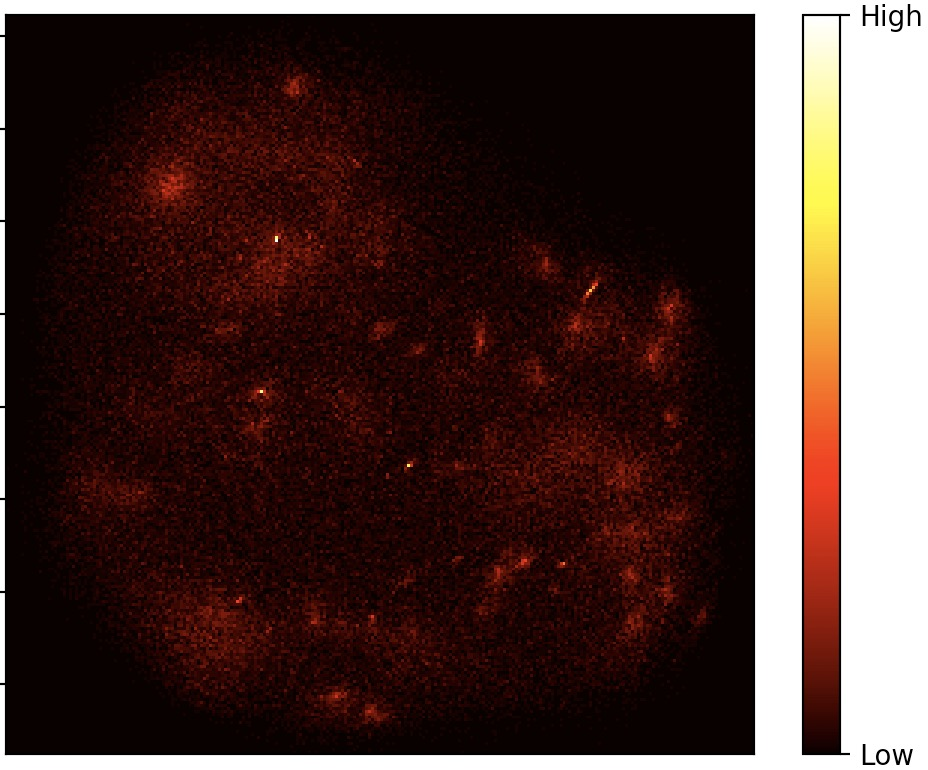
\includegraphics[width=\textwidth]{heatmap}
  \caption{Heat map of the Dimred dataset. The lighter versions of the figure are for} 
  \label{fig:heatmap}
\end{figure}

We can clearly see that the new new seeding process gave us marginally better results than \kmeans in some situations. In most cases, it did equally as bad if not worse. We also note that \kmeansn ++ did considerably better in most cases. From that we conclude that the new seeding process is no better than \kmeans.

It is important to note here that on the dimred dataset, unlike the other datasets, all three algorithms achieve similar results. 











\section{Minimum Weight Perfect Matching on Bipartite Graphs}
In an effort to understand the robustness of the algorithms, we decided to see how consistent the results of the algorithm were were multiple consecutive runs. For that, we used the Hungarian algorithm for perfect matching introduced by\cite{kuhn}. We learned a lot about the underlying properties of the algorithm by analyzing our perfect matching results. First, we realized how perfectly matching two runs of the algorithm does not necessarily mean perfectly matching the centres based on their distances in euclidean space. Second, minimizing the total distance between pairs in the matching may not be the best way to best match the centres.

Perfect matching is the problem where a graph is partitioned into pairs based on a heuristic. Minimum weight perfect matching is where the total costs of the edges connecting the pairs in the graph are minimized. The is an NP-hard problem on a general graph; however, it can be solved in $O(n^3)$. The Hungarian algorithm is one of the best known problems to solve the assignment problem, the more widely used name of the minimum weight perfect matching problem.

The assignment problem is where given a set of w workers and t tasks, we are asked to find the best worker-pair pairing so that the total cost to perform all tasks is minimized.

\begin{figure}[h]
  \begin{subfigure}[b]{0.5\textwidth}
    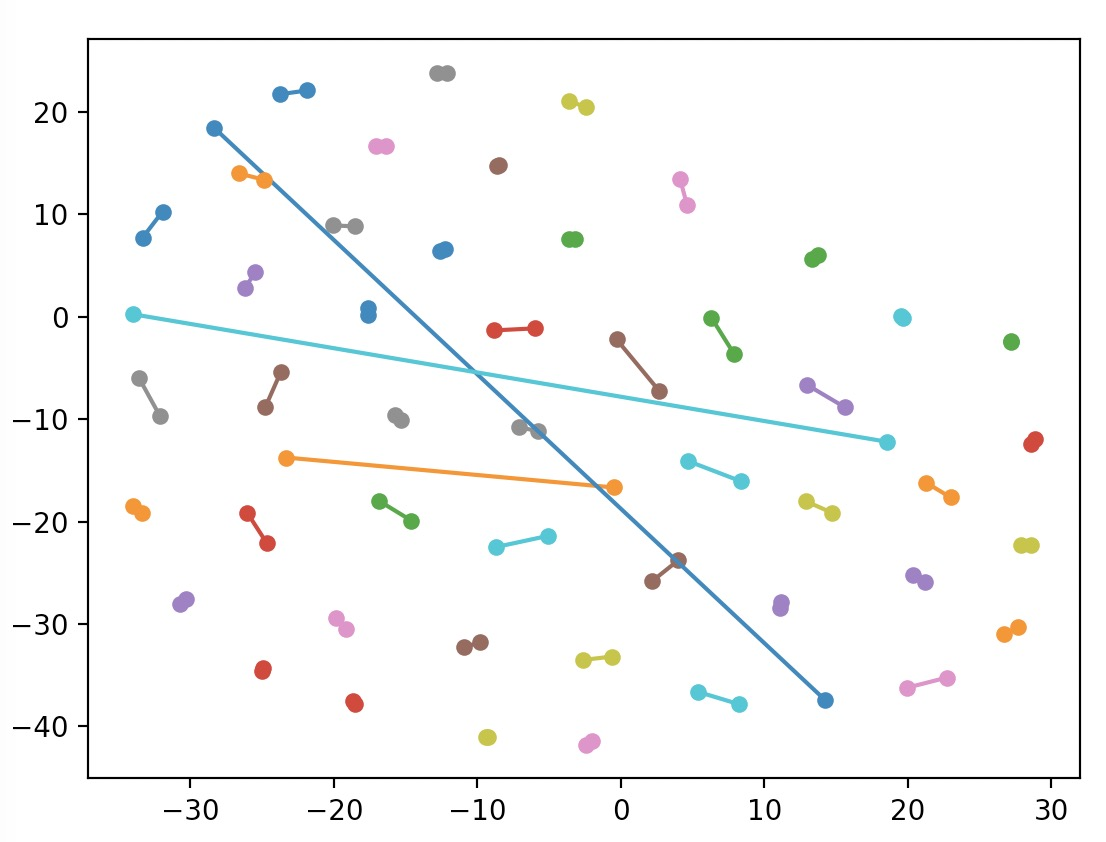
\includegraphics[width=\textwidth]{overlap}
    \caption{Perfect matching using maximum overlap of points in centres}
    \label{fig:overlap}
  \end{subfigure}
  \begin{subfigure}[b]{0.5\textwidth}
    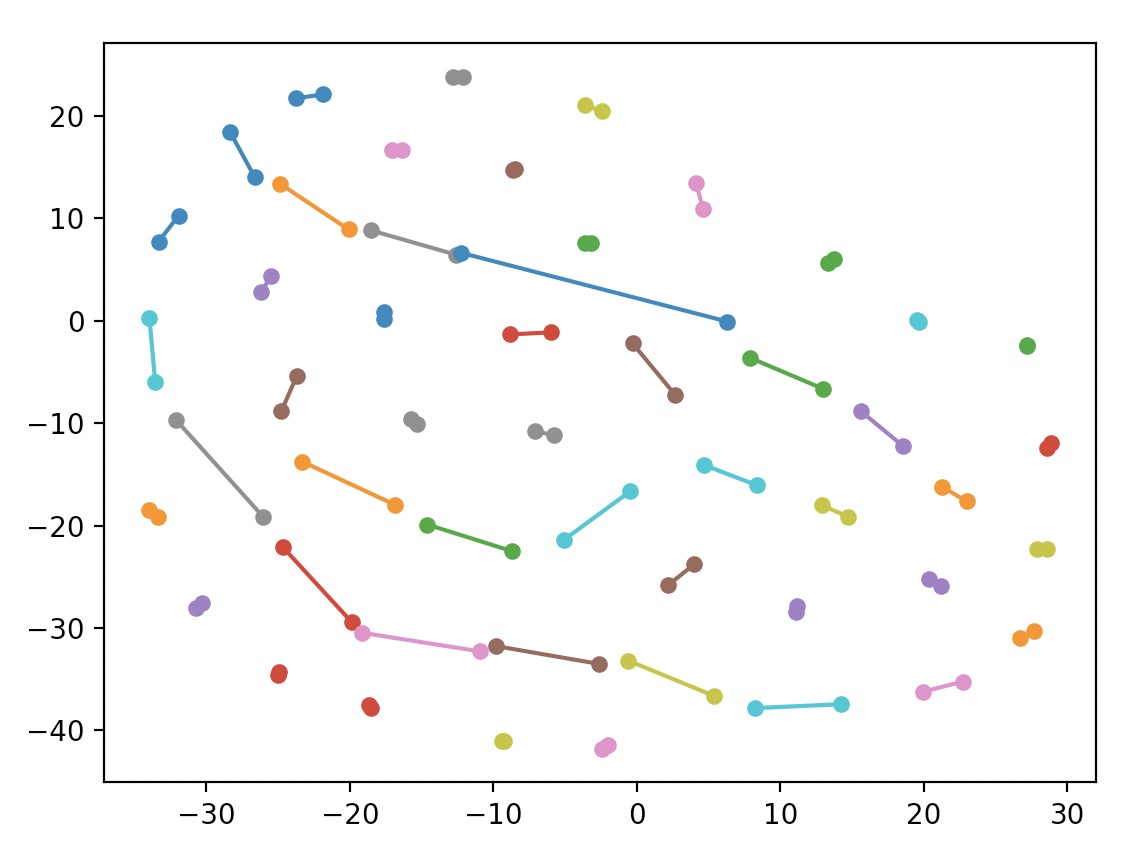
\includegraphics[width=\textwidth]{distance}
    \caption{Perfect matching using distances of cluster centres to each other.}
    \label{fig:distance}
  \end{subfigure}
  \caption{Example of different cost functions for perfect matching.}
\end{figure}

The two figures are of clusters centres plotted in euclidean space. The axis are not labeled because it adds no extra information to our findings in this case. Every pairing of same-colour points on the plots come from $2$ different runs of the algorithm. We perfectly match the 100 points (50 per run), and get some interesting results.

Here we can see Figures ~\ref{fig:overlap} \& ~\ref{fig:distance} are very different even though they are run on the same datasets. There is a very good explanation for this that may not be clear at first glance. Figure ~\ref{fig:distances} seems to be inaccurate as there are clear pairings of points that weren't paired together. Rather than the closest points being paired, we see how there is a chain of pairings. This is because running the minimum weight perfect matching on the points minimizes the overall distances between all the pairs, but does not take into consideration the actual underlying pairing that we are looking for.

Switching the objective function in Figure \ref{fig:overlap} where we compute the maximum weight perfect matching of the centres based on the number of shared points in the clusters. Here, we notice a very interesting pattern where the pairings seem to be near perfect overall with a few outliers that is far apart. While this is not exactly the expected result, it makes sense because for this dataset, we are not sure of the exact underlying number of clusters k. 

% TODO: finish this part explaining why there are points that are very far apart that are matched


\section{Choosing the Correct Matching Function}
In our experiments, we were looking to perfectly match 50 centres on multiple runs of the algorithm on the
% TODO: Add dataset name:
 dataset. To do that we initially computed the distances between every pair of cluster centres and ran the minimum-weight perfect matcher on that. We got the following result.
%  TODO: Add picture of the centres being perfectly matched.

The objective function was later changed to maximum-weight perfect matching based on the number of shared points between clusters. Here, a very interesting property was observed. Most of the points were perfectly matched while the rest were 


\chapter{Extendable C++ Implementation}

Throughout the research for this paper, it was difficult to find modular code that is easily extendable for the \kmeans algorithm that allow us to perform testing on it. For that, we created our own implementation that is available on Github \cite{YaserKmeans}. This implementation is free to use and licenced under the MIT License, allow users to modify it as they see fit without any warranty on functionality or fitness for a particular purpose.

The algorithm is implemented in highly optimized C++ with object oriented programming at its core. This allows other developers to extend the algorithm and test different combinations of optimizations in the code. It can be used by both individuals needing to use a \kmeans implementation and ones who are looking to do research and optimize it further. 

Every \kmeans instance, contains templated instances of a SeedPicker and an IterationRunner along with a skeleton that allows analysis of the performance of each run of the algorithm. This allows us to use different IterationRunners and SeedPickers interchangeably in the algorithm depending on the algorithm at hand and the resources allowed. The analytical data being saved at each run is independent of the SeedPicker and IterationRunner, which makes it simple for developers wanting to extend the algorithm.

The modularity of the implementation also allows developers to create new SeedPicker and IterationRunner classes. To create one, all they are required to do is implement a function from their respective Base class. For example, the $kd$-tree implementation of the algorithm has be hooked into a \kmeans instance by implementing it as an IterationRunner.


\chapter{Conclusion}

\kmeans is a problem that has proven to be applicable to many domains and applications. It is still widely used and continues to be so. We have shown that the new \kmeansn Consensus method of seeding the \kmeans algorithm is no better than randomly seeding the algorithm. 

One area of research that is needed is a way to compute the real number $k$ for the algorithm. We have a method to compute that by calculating cliques in perfectly matched centres over multiple runs of the algorithm, but this needs further exploration. 




\bibliographystyle{newapa}
\bibliography{yaser_thesis}

\end{document}





% \begin{figure}[h!]
%   \begin{minipage}{0.48\textwidth}
%   \begin{center}
%     \begin{tikzpicture}
%       \begin{axis}[
%         width=\linewidth, % Scale the plot to \linewidth
%         grid=major, % Display a grid
%         grid style={dashed,gray!30}, % Set the style
%         xlabel=X Axis, % Set the labels
%         ylabel=Y Axis,
%         legend style={at={(0.5,-0.3)},anchor=north} % Put the legend below the plot
%         % x tick label style={rotate=90,anchor=east} % Display labels sideways
%       ]
%       \addplot+[mark options={scale=0.1}] table[only marks,col sep=comma] {plotData/dataset0-cluster-0.csv};
%       \addplot+[mark options={scale=0.1}] table[only marks,col sep=comma] {plotData/dataset0-cluster-1.csv};
%       \addplot+[mark options={scale=0.1}] table[only marks,col sep=comma] {plotData/dataset0-cluster-2.csv};
%       \addplot+[mark options={scale=0.1}] table [only marks,col sep=comma] {plotData/dataset0-cluster-3.csv};
%       \legend{Cluster}
%     \end{axis}
%     \end{tikzpicture}
%     \caption{My firsts autogenerated plot.}
%   \end{center}
% \end{minipage}\hfill
% \begin {minipage}{0.48\textwidth}
%   \begin{center}
%     \begin{tikzpicture}
%       \begin{axis}[
%         width=\linewidth, % Scale the plot to \linewidth
%         grid=major, % Display a grid
%         grid style={dashed,gray!30}, % Set the style
%         xlabel=X Axis, % Set the labels
%         ylabel=Y Axis,
%         legend style={at={(0.5,-0.3)},anchor=north} % Put the legend below the plot
%         % x tick label style={rotate=90,anchor=east} % Display labels sideways
%       ]
%       \addplot+[mark options={scale=0.1}] table[only marks,col sep=comma] {plotData/dataset1-cluster-0.csv};
%       \addplot+[mark options={scale=0.1}] table[only marks,col sep=comma] {plotData/dataset1-cluster-1.csv};
%       \addplot+[mark options={scale=0.1}] table[only marks,col sep=comma] {plotData/dataset1-cluster-2.csv};
%       \addplot+[mark options={scale=0.1}] table [only marks,col sep=comma] {plotData/dataset1-cluster-3.csv};
%       \legend{Cluster}
%     \end{axis}
%     \end{tikzpicture}
%     \caption{My second autogenerated plot.}
%   \end{center}
% \end{minipage}\hfill
% \end{figure}